\documentclass[conference]{IEEEtran}
\IEEEoverridecommandlockouts

\usepackage{cite}
\usepackage{amsmath,amssymb,amsfonts}
\usepackage{graphicx}
\usepackage{booktabs}
\usepackage{xcolor}
\usepackage[hyphens]{url}
\usepackage[colorlinks=true,linkcolor=blue,citecolor=blue,urlcolor=blue]{hyperref}

\graphicspath{{../figures/}}

\begin{document}
\bstctlcite{IEEEexample:BSTcontrol}

\title{Allele Frequency, Linkage Disequilibrium, or Effect Size? Decomposing Cross-Ancestry Disagreement in Genetically Regulated Expression Models, with Application to Autism and Psychiatric TWAS}

\author{\IEEEauthorblockN{Kehinde Obidele}
\vspace{12.8pt}
\IEEEauthorblockA{\textit{Department of Health Informatics, Northeastern University}}}

\maketitle

\begin{abstract}
Genetically regulated expression models trained in one ancestry predict poorly in another, but it is not clear which of three ingredients is responsible: the model weights, the allele frequencies of the variants used, or the linkage disequilibrium among them. This study decomposes the difference in genetically regulated variance between two ancestry-specific models into exactly these three parts using a Shapley decomposition, which is order-independent and sums to the total for every gene. Elastic-net models were trained on GEUVADIS lymphoblastoid expression for 358 European and 87 Yoruba individuals with 1000 Genomes phase 3 genotypes, with European sets downsampled to 87 to separate sample size from ancestry. The weights term is by far the largest, with a median absolute value of 0.75 against 0.25 for allele frequency and 0.13 for linkage disequilibrium. Measured against a within-ancestry control built from independent European draws, in which the frequency and LD terms are zero by construction, about 70\% of that weights term is reproduced by resampling a single population, and its noise floor, between 0.54 and 0.61 across three pairs of European draws, exceeds the other two terms combined. The two smaller terms point in consistent directions across genes and each tracks the genotype quantity it is named for. Applying both model sets to autism and four psychiatric disorders, 76\% of associations found with one ancestry's models and not the other involve genes the other ancestry could not model at all, and allele frequency is the largest component for 4 of 129 such associations. Cross-population accuracy is governed mainly by whether the two ancestries selected the same variants.
\end{abstract}

\begin{IEEEkeywords}
transcriptome-wide association study, genetically regulated expression, genetic ancestry, linkage disequilibrium, allele frequency, Shapley decomposition, autism spectrum disorder, psychiatric genetics
\end{IEEEkeywords}

\section{Introduction}

Transcriptome-wide association studies (TWAS) link genetic risk to genes by predicting gene expression from genotype and testing the predicted expression for association with disease~\cite{gamazon2015,gusev2016,barbeira2018}. The prediction models behind TWAS are trained on reference panels that pair genotypes with RNA sequencing, and those panels come overwhelmingly from people of European ancestry~\cite{gtex2020,wang2018}. The same imbalance runs through human genetics as a whole~\cite{popejoy2016,sirugo2019}, even though African genomes carry the greatest genetic diversity of any population~\cite{campbell2008,gurdasani2015}.

It is well established that expression models lose accuracy when carried from one ancestry to another~\cite{mogil2018,mikhaylova2019,keys2020}. It is much less clear why. A model trained in one population can disagree with a model trained in another because the regulatory effects differ, because the variants it relies on are common in one population and rare in the other, or because linkage disequilibrium (LD) makes different variants good proxies for the same causal signal. These explanations have different consequences. If effects differ, models from each ancestry are required. If allele frequency or LD is the main source, better variant coverage and more careful choice of predictors can recover much of the loss.

This study separates those explanations exactly. For any model, the variance of genetically regulated expression depends on three ingredients: the model weights, the allele frequencies of the variants it uses, and the LD among them. Each ingredient can be taken from either population, which turns the difference between a European-trained and a Yoruba-trained model into a three-way decomposition with a unique fair split, the Shapley value~\cite{shapley1953,owen2014}. We applied it to elastic-net expression models trained at equal sample size in European and Yoruba lymphoblastoid cell lines from GEUVADIS~\cite{lappalainen2013}, measured how much of each model's accuracy survives in the other population, and followed the consequences into TWAS of autism and four psychiatric disorders.

The study makes four contributions. First, an exact decomposition of cross-ancestry model disagreement into weight, allele frequency and LD components, computed for every gene with usable models in both ancestries. Second, a within-ancestry noise floor, built from independent European draws of the same size, against which the weight component is read, so that training noise is not mistaken for biology. Third, transfer accuracy for every usable model in both directions, benchmarked against published estimates. Fourth, the practical consequence for association studies: how often the two model sets agree on which genes are associated with autism, schizophrenia, bipolar disorder, major depression and post-traumatic stress disorder, and how much of a Yoruba model's signal a European GWAS can measure at all.

\section{Related Work}

\subsection{Transcriptome-Wide Association Methods}
PrediXcan introduced gene-level association through predicted expression~\cite{gamazon2015}, and FUSION developed a closely related approach for summary statistics~\cite{gusev2016}. S-PrediXcan made PrediXcan usable with GWAS summary statistics alone~\cite{barbeira2018}, and MultiXcan combined predictions across tissues~\cite{barbeira2019}. Summary-data Mendelian randomization offered a complementary route from eQTL and GWAS data to candidate genes~\cite{zhu2016}. As TWAS spread, its limits became clearer: associations can arise from LD with a nearby causal gene or from shared regulation rather than from the tested gene itself~\cite{wainberg2019}, which motivated fine-mapping methods that model correlated predicted expression jointly~\cite{mancuso2019}. The expression models in these tools are usually elastic-net regressions~\cite{zou2005,friedman2010} trained on residual expression after removing technical and population structure, often with PEER factors~\cite{stegle2012}.

\subsection{Transferring Genetic Prediction Across Ancestries}
For polygenic scores, the loss of accuracy across ancestries is well documented~\cite{martin2017,martin2019,duncan2019}. Theory and data show that differences in allele frequency and LD between the training and target populations reduce accuracy even when causal effects are shared~\cite{wang2020}, and that accuracy declines steadily with genetic distance from the training data, even within populations usually treated as homogeneous~\cite{ding2023}. Genetic correlation estimates across ancestries suggest that causal effects are largely, but not entirely, shared~\cite{brown2016}, and population-specific effect sizes are concentrated in functionally important regions affected by selection~\cite{shi2021}. Studies of more diverse samples have shown that this diversity improves discovery~\cite{wojcik2019}.

For gene expression, cis-regulatory variation differs across populations~\cite{stranger2012}, and expression models trained in one population predict poorly in others~\cite{mogil2018}. Accuracy also varies within continental groups~\cite{mikhaylova2019}. Keys et al. trained elastic-net models on GEUVADIS populations downsampled to the size of the Yoruba sample and found that European-trained models explained on average about 5\% of expression variance in African individuals, with simulations indicating that transfer succeeds only when eQTL architecture is shared~\cite{keys2020}. Recent work shows that combining ancestries in training increases TWAS discovery~\cite{bledsoe2026}. In brain, Jajoo et al. trained ancestry-specific expression models from PsychENCODE and found that weights on shared predictors correlated at $r = 0.6$ with 97\% agreement in sign, and that most associations detected in only one ancestry involved variants with lower allele frequency in the other~\cite{jajoo2025}.

\subsection{Gap Addressed by This Study}
These studies measure how much accuracy is lost and point to allele frequency and LD as likely causes, but they do not assign the disagreement between two models to its sources in a way that sums exactly to the total. They also rarely separate genuine cross-ancestry differences from the disagreement that arises between two models trained on different samples of the same population. This study provides both, using a decomposition with a closed form for each gene, and connects the result to psychiatric TWAS.

\subsection{Expression Resources for Psychiatric Genetics}
Brain expression resources have shown that psychiatric disorders share molecular signatures that track their genetic overlap~\cite{gandal2018,wang2018}, and TWAS of schizophrenia has prioritized genes and regulatory mechanisms at many risk loci~\cite{gusev2018}. The psychiatric GWAS used here~\cite{grove2019,trubetskoy2022,mullins2021,adams2025,nievergelt2024} are among the largest available, and all were analyzed in European-ancestry samples.

\section{Methods}

\subsection{Data}
Gene expression came from the GEUVADIS project~\cite{lappalainen2013}, which sequenced mRNA from lymphoblastoid cell lines (LCLs) of 462 individuals drawn from five 1000 Genomes populations. This study used the released gene-level RPKM matrix. Genotypes came from 1000 Genomes phase 3~\cite{kg2015} on GRCh37, processed with PLINK 2~\cite{chang2015}. Of the 462 individuals with expression data, 445 have phase 3 genotypes; the other 17 appear in earlier 1000 Genomes releases but not in phase 3. The analytic sample was therefore 358 individuals of European ancestry (FIN 92, TSI 91, CEU 89, GBR 86) and 87 Yoruba individuals from Ibadan, Nigeria (YRI).

GWAS summary statistics came from the Psychiatric Genomics Consortium for five traits: autism spectrum disorder (18,381 cases, 27,969 controls)~\cite{grove2019}, schizophrenia (European meta-analysis, 52,017 cases, 75,889 controls)~\cite{trubetskoy2022}, bipolar disorder (41,917 cases, 371,549 controls)~\cite{mullins2021}, major depression (European ancestry, excluding 23andMe, 412,305 cases, 1,588,397 controls)~\cite{adams2025}, and post-traumatic stress disorder (European ancestry, 137,136 cases, 1,085,746 controls)~\cite{nievergelt2024}. All five are of European ancestry and on GRCh37.

\subsection{Training Sets}
Three kinds of training set were built from the 445 individuals (Fig.~\ref{fig:design}). EUR358 contains every European individual and YRI87 every Yoruba individual. EUR87 is a random draw of 87 European individuals, repeated with five random seeds. Comparing EUR358 with EUR87 isolates the effect of sample size, and comparing EUR87 with YRI87 compares the two ancestries at equal sample size.

\subsection{Genotype and Expression Processing}
Genotypes were restricted to biallelic autosomal single-nucleotide variants (SNVs) with minor allele frequency (MAF) of at least 0.01 in either population. This left 17,342,935 SNVs: 6,315,760 common in both samples, 8,794,594 common only in the Yoruba sample, and 2,232,581 common only in the European sample. Genotype principal components were computed within each population on LD-pruned SNVs (MAF $\geq 0.05$, $r^2 < 0.2$ within 1 Mb windows).

Expression was processed separately within each training set, so that each European draw received exactly the treatment the Yoruba set received. Within a set, autosomal genes with RPKM above 0.1 in at least 20\% of individuals were retained (20,747 to 20,799 genes per set). Each gene was rank-based inverse-normal transformed and residualized on sex, three genotype principal components, and $K$ expression principal components, used in place of PEER factors~\cite{stegle2012}, with $K = 15$ for $n = 358$ and $K = 5$ for $n = 87$.

\subsection{Elastic-Net GReX Models}
For each gene, predictors were cis SNVs within 500 kb of the gene coordinate with MAF of at least 0.05 in the training set. Models were fit with elastic net~\cite{zou2005} ($\alpha = 0.5$) in glmnet~\cite{friedman2010}. Prediction performance was estimated by nested cross-validation: five outer folds, and within each outer training portion, $\lambda$ chosen by five-fold cross-validation. The cross-validated $R^2$ is the squared Pearson correlation between held-out predictions and observed expression across all individuals. Final weights came from a fit on all individuals, again with $\lambda$ chosen by five-fold cross-validation. Following PredictDB conventions~\cite{gamazon2015,barbeira2018}, a model was considered usable when its cross-validated $R^2$ exceeded 0.01 with $p < 0.05$ and its final fit retained at least one non-zero weight.

The 500 kb window and the MAF floor of 0.05 are stricter than the common 1 Mb and 0.01 defaults. At $n = 87$, a variant with MAF 0.01 is carried by only two to eight chromosomes, too few for a stable weight, and applying the same floor to every set keeps the comparisons fair. The stricter settings also reduced the computation to a size that could be run on a single workstation.

\subsection{Variance Decomposition}
For a model with weights $w$ over a set of SNVs, the variance of genetically regulated expression in a population with allele frequencies $p_j$ and LD correlation matrix $R$ is
\begin{equation}
V(w, D, R) = w^{\top} D^{1/2} R\, D^{1/2} w, \quad D = \mathrm{diag}\big(2 p_j (1 - p_j)\big).
\label{eq:variance}
\end{equation}
Equation~\eqref{eq:variance} depends on three ingredients that can each be taken from either population: the weights $w$, the frequencies $D$, and the LD structure $R$. For each gene with usable European and Yoruba models, weights were placed on the union of SNVs selected by either model (zero where a model did not select a SNV). $D$ and $R$ were computed from the full EUR358 and YRI87 genotypes, so the frequency and LD ingredients do not depend on which European draw trained the model. The gap between ancestries is
\begin{equation}
\Delta = \log V(w_Y, D_Y, R_Y) - \log V(w_E, D_E, R_E).
\label{eq:gap}
\end{equation}
Let $v(S)$ denote $\log V$ with the ingredients in $S \subseteq \{w, D, R\}$ taken from the Yoruba sample and the rest from the European sample. The Shapley value~\cite{shapley1953,owen2014} assigns ingredient $k$ the contribution
\begin{equation}
\phi_k = \sum_{S \subseteq \{w,D,R\} \setminus \{k\}} \frac{|S|!\,(2 - |S|)!}{3!}\,\big[v(S \cup \{k\}) - v(S)\big],
\label{eq:shapley}
\end{equation}
which averages the effect of swapping $k$ over all six orders in which the three ingredients can be swapped. The contributions sum exactly to the gap, $\phi_w + \phi_D + \phi_R = \Delta$, and this identity was checked numerically for every gene. Genes for which some mixed combination has $V = 0$, because all weight sits on SNVs monomorphic in the other sample, cannot be placed on the log scale and are reported separately.

\subsection{Within-Ancestry Noise Floor}
Two models trained on different samples of the same population also disagree, because elastic net fits noise and, among correlated SNVs, keeps one tag somewhat arbitrarily. Without a reference point, that disagreement would be attributed to ancestry. The decomposition was therefore also run between independent European draws (EUR87, seeds 1 and 2, and subsequently seeds 1 and 3 and seeds 2 and 3), with $D$ and $R$ taken from the EUR358 genotypes for every model. In that comparison $\phi_D = \phi_R = 0$ by construction, and $\Delta = \phi_w$ measures how much weight disagreement arises from training on 87 individuals alone. Cross-ancestry weight components are interpreted only relative to this floor.

\subsection{Prediction Agreement}
Because two models can capture the same regulatory signal through different tag SNVs, weight comparisons alone can overstate disagreement. For each gene, both models were applied to the same individuals and the Pearson correlation between their predictions was computed, once in the European genotypes and once in the Yoruba genotypes. High agreement with few shared SNVs indicates that the models differ in tag choice rather than in the genetic signal they capture.

\subsection{Cross-Population Prediction}
Each European model was applied to the Yoruba genotypes and its predictions correlated with the Yoruba individuals' adjusted expression, and each Yoruba model was applied to the European sample in the same way. Accuracy in the other population is reported as a signed $r^2$, negative when a model's predictions run opposite to the observed expression.

The drop from a model's accuracy at home to its accuracy in the other population is deliberately not used as an outcome anywhere in this study. Home accuracy is a nested cross-validation estimate, in which every fold is fitted on a subset of the training individuals, while the cross-population figure comes from the final model fitted on all of them and evaluated in an independent sample. The two are not the same kind of estimate, and their difference is negative for 28.5\% of genes in one direction and 47.6\% in the other, tracking the number of SNVs the two models share rather than any property of the populations.

Cross-population accuracy was instead related directly to three per-gene quantities: the number of SNVs both models selected, a weight-averaged frequency divergence, and a weight-averaged LD divergence. Writing $a_j$ for the normalized sum of the absolute weights of SNV $j$ in the two models, so that $\sum_j a_j = 1$, and $\bar{p}_j = (p_{Ej} + p_{Yj})/2$, the frequency term is Nei's fixation index averaged over the SNVs a model uses,
\begin{equation}
F_{\mathrm{ST}}^{(w)} = \sum_j a_j \frac{(p_{Ej} - p_{Yj})^2}{4\,\bar{p}_j (1 - \bar{p}_j)},
\label{eq:fst}
\end{equation}
and the LD term is
\begin{equation}
L^{(w)} = \frac{\sum_{i \neq j} a_i a_j \, |R_{E,ij} - R_{Y,ij}|}{\sum_{i \neq j} a_i a_j}.
\label{eq:lddiv}
\end{equation}
Equation~\eqref{eq:fst} is an average of per-SNV ratios rather than the ratio of averages usually preferred for combining $F_{\mathrm{ST}}$ across variants, and it is computed only over SNVs a model selected, all of which passed a minor allele frequency floor of 0.05 in their training sample. It is therefore a model-weighted summary and not a genome-wide figure.

Each quantity was related to cross-population accuracy by a partial Spearman correlation holding the model's own cross-validated accuracy at home fixed, computed on ranks with the control regressed out, with 95\% intervals from 800 bootstrap resamples of genes.

\subsection{GWAS Harmonization}
For each GWAS, a $z$-score was computed for the reported effect allele and aligned to the ALT allele of the 1000 Genomes variant with the same position and alleles. Palindromic SNVs (A/T and C/G) were removed. The PGC schizophrenia and bipolar files code the reference allele as A1 in every row, so every $z$ changed sign during alignment. This convention was confirmed rather than assumed: on chromosome 22 the files' control allele frequency correlated at $r = 0.997$ with the 1000 Genomes European frequency of A1. As an independent check on sign, pairwise correlations of the aligned $z$-scores across roughly 5.5 million shared SNVs (excluding the MHC and the 17q21.31 inversion) were positive for every pair of traits, and highest for schizophrenia and bipolar disorder ($r = 0.375$), as expected from their genetic correlation.

\subsection{Summary-Statistic TWAS}
Gene-level association was computed in the S-PrediXcan form~\cite{barbeira2018},
\begin{equation}
z_g = \sum_{j} w_j \frac{\sigma_j}{\sigma_g} z_j, \qquad \sigma_g^2 = w^{\top} \Sigma\, w,
\label{eq:twas}
\end{equation}
where $\Sigma$ and $\sigma_j$ come from the EUR358 genotypes because all five GWAS are European. SNVs absent from a GWAS were dropped from that trait's sum and from $\sigma_g$. Coverage was recorded as the share of a model's variance that remains after this restriction. The implementation was validated against the official S-PrediXcan software on the Yoruba chromosome 22 models: gene $z$-scores agreed with Pearson $r = 1.000$ and a maximum absolute difference of $1.5 \times 10^{-7}$ across 62 genes for schizophrenia and $4.5 \times 10^{-8}$ across 61 genes for autism. The two implementations selected identical SNV sets for every autism gene and for 98.4\% of the schizophrenia genes, so the residual differences reflect both arithmetic precision and a small number of genes where SNV selection differed. Associations were declared significant at a Bonferroni threshold within each trait and model set, with Benjamini-Hochberg false discovery rates reported alongside.

\section{Results}
\begin{figure*}[!t]
\centering
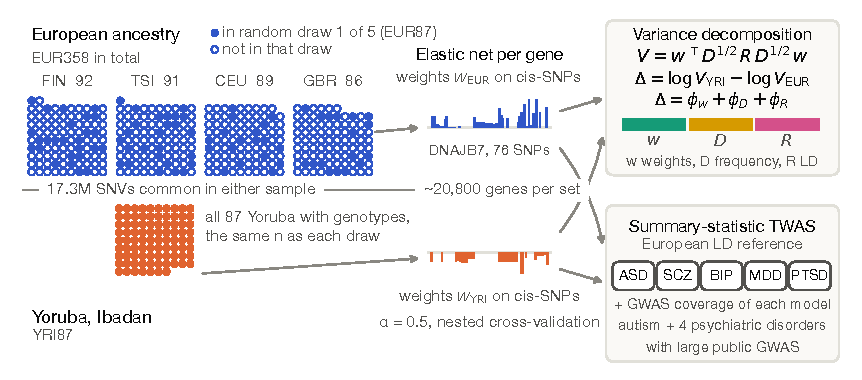
\includegraphics[width=\textwidth]{fig01_design}
\caption{Design of the study. The 445 individuals with both expression and phase 3 genotypes are drawn one dot per person, European above the axis and Yoruba below. Filled European dots are the 87 individuals in random draw 1; the same draw was repeated five times. The stems are the real elastic-net weights for DNAJB7, a gene examined in detail later, with the European model above and the Yoruba model below. Every pair of models feeds the variance decomposition and the summary-statistic TWAS.}
\label{fig:design}
\end{figure*}


\subsection{Two Samples, Different Genetic Ground}
Of the 17,342,935 SNVs common (MAF $\geq 0.01$) in at least one sample, 6,315,760 (36\%) were common in both, 8,794,594 (51\%) only in the Yoruba sample, and 2,232,581 (13\%) only in the European sample (Fig.~\ref{fig:landscape}). Put the other way round, 58\% of the SNVs common in the Yoruba sample were not common in the European sample, while 26\% of the European sample's common SNVs were not common in the Yoruba sample. The Yoruba-only share was fairly uniform across the genome (mean 0.51, standard deviation 0.054 across 2,725 one-megabase tiles). The clearest exception was the major histocompatibility complex on chromosome 6, where the Yoruba-only share fell to 8.5\% in the tile at 32 Mb, the lowest in the genome, consistent with HLA alleles that are kept common in every population.
\begin{figure*}[!t]
\centering
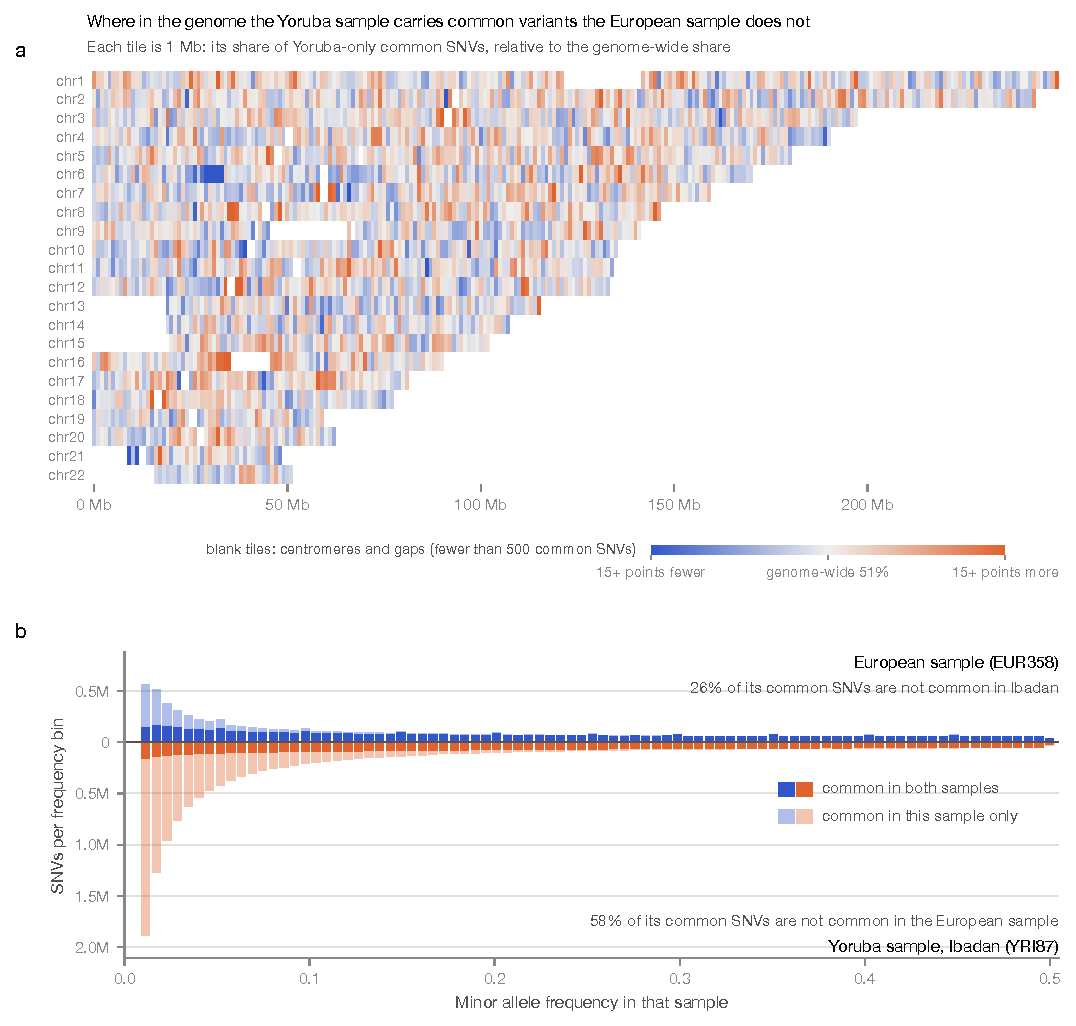
\includegraphics[width=\textwidth]{fig02_frequency_landscape}
\caption{The genetic ground each sample stands on. (a) Every one-megabase tile of the autosomes, colored by how far its share of Yoruba-only common SNVs departs from the genome-wide 51\%. Blank tiles are centromeres and assembly gaps with fewer than 500 common SNVs. The deep blue block on chromosome 6 is the major histocompatibility complex. (b) Allele-frequency spectrum of common SNVs, European above the axis and Yoruba below, with the darker fill marking variants common in both samples.}
\label{fig:landscape}
\end{figure*}


Linkage disequilibrium was weaker in the Yoruba sample at equal sample size (Fig.~\ref{fig:ld}). Across chromosome 22, mean $r^2$ between SNVs 0.5 kb apart was 0.54 in a draw of 87 European individuals and 0.42 in the 87 Yoruba individuals, and 0.21 versus 0.13 at about 16 kb. Around DNAJB7, the gene examined in detail below, mean pairwise $r^2$ among 150 SNVs common in both samples was 0.33 in the European draw and 0.22 in the Yoruba sample.
\begin{figure*}[!t]
\centering
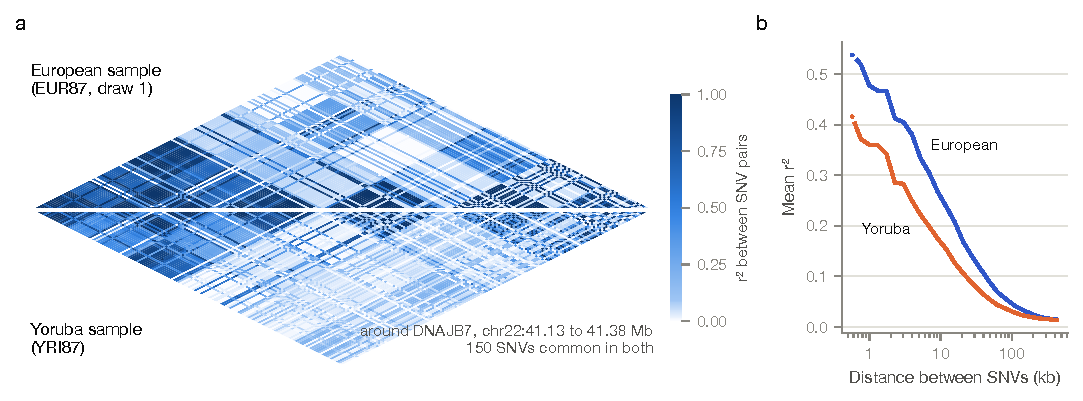
\includegraphics[width=\textwidth]{fig03_ld_decay}
\caption{Linkage disequilibrium decays faster in the Yoruba sample. (a) Pairwise $r^2$ among the 150 SNVs common in both samples around DNAJB7, European above and Yoruba below the midline, on a common linear scale. (b) Mean $r^2$ against distance between SNVs across chromosome 22, both computed at $n = 87$.}
\label{fig:ld}
\end{figure*}


\subsection{Similar Yield, Different Genes}
At equal sample size the two ancestries produced almost the same number of usable models: 2,286 genes for the European draw (median cross-validated $R^2 = 0.081$) and 2,230 for the Yoruba sample (median 0.078; Fig.~\ref{fig:accuracy}). Genes with strong, well-known lymphoblastoid eQTLs were recovered in the Yoruba sample, including ERAP2 ($R^2 = 0.59$), HLA-DQA1 (0.42) and PEX6 (0.31), which supports the pipeline end to end.
\begin{figure*}[!t]
\centering
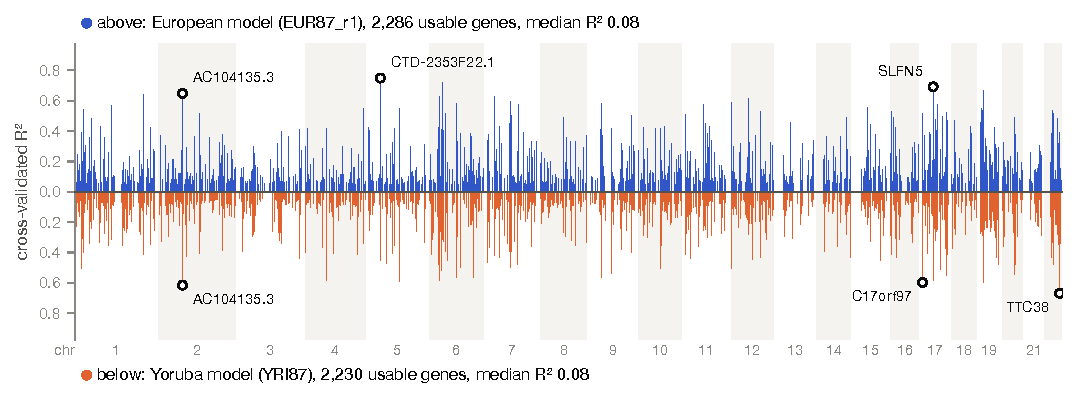
\includegraphics[width=\textwidth]{fig05_accuracy_mirror}
\caption{Cross-validated accuracy along the genome, one stem per usable model at its gene position, the European draw above the axis and the Yoruba sample below. Alternating bands separate chromosomes. The named genes are the strongest models in each direction, chosen at least 200 Mb apart.}
\label{fig:accuracy}
\end{figure*}


The two models did not, however, find the same genes (Fig.~\ref{fig:concordance}). Of 20,619 genes fit in both sets, only 562 were usable in both, while 1,710 were usable only with the European model and 1,645 only with the Yoruba model. Across all genes the rank correlation of cross-validated $R^2$ was 0.04, because most genes sit near zero in both samples, where cross-validated $R^2$ is dominated by noise. Among the 562 genes usable in both, it was 0.50. The two samples therefore broadly agree on how predictable a gene is when both can predict it, but at 87 individuals each they reach usable models for largely different sets of genes.
\begin{figure}[!t]
\centering
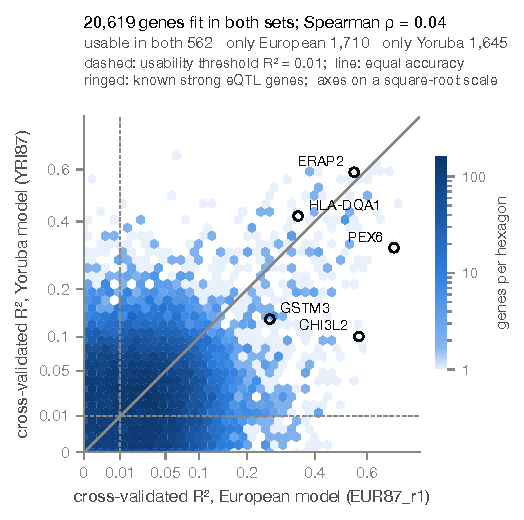
\includegraphics[width=\columnwidth]{fig06_r2_concordance}
\caption{Do the two samples agree on which genes are predictable? Log-density of cross-validated $R^2$ for the 20,619 genes fit in both sets, on square-root axes. Dashed lines mark the usability threshold of $R^2 = 0.01$ and the solid line marks equal accuracy. Ringed points are genes with strong, well-known lymphoblastoid eQTLs.}
\label{fig:concordance}
\end{figure}


One property of small training sets shaped these counts. In the Yoruba sample, 6,112 genes passed the cross-validation criteria, but for 3,882 of them (64\%) the final elastic-net fit on all 87 individuals selected no SNVs, because the penalty chosen by cross-validation on the full sample fell at the intercept-only end of the path. Such genes cannot be used for prediction or TWAS, and this limit on usable models applies equally to both ancestries at this sample size.

The yield itself barely depends on ancestry once sample size is held equal (Fig.~\ref{fig:yield}). Two further independent draws of 87 Europeans produced 2,219 and 2,351 usable models, so the three European draws span 2,219 to 2,351 and the Yoruba count of 2,230 falls inside that range. The difference between random draws of one population is therefore larger than the difference between populations. The same holds at every stage of the funnel: 6,112 to 6,799 genes clear cross-validation in each set, and roughly two thirds of those are then lost to an empty final fit, in every set alike.

\begin{figure*}[!t]
\centering
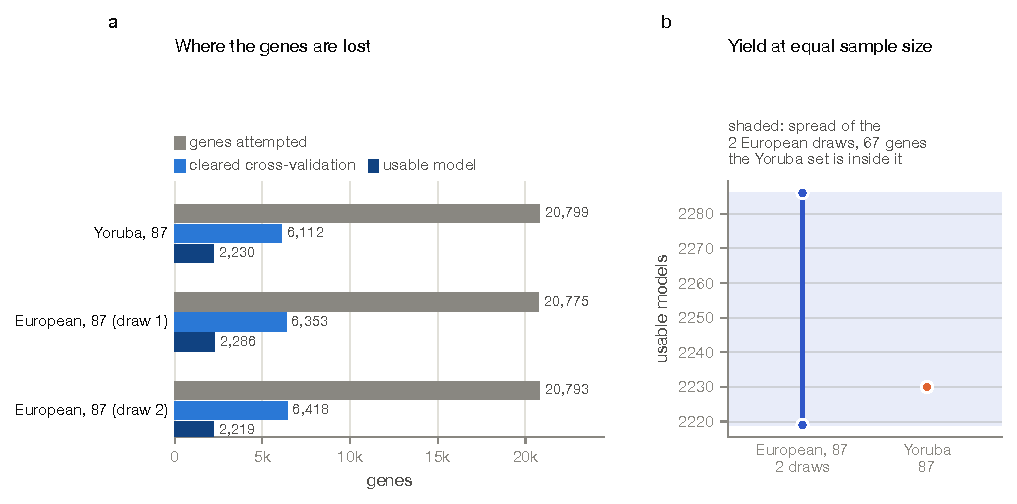
\includegraphics[width=\textwidth]{fig04_yield}
\caption{Model yield. (a) For each training set, the genes attempted, those clearing the cross-validation criteria, and those retaining a usable model after the final fit. (b) Usable models per set. The shaded band is the spread between the European draws of 87, against which the Yoruba count can be read directly.}
\label{fig:yield}
\end{figure*}

\subsection{What Sample Size Alone Buys}
Training on more individuals of the same ancestry changed both how many genes could be modelled and how well each one was predicted (Fig.~\ref{fig:samplesize}). With all 358 Europeans, 5,524 genes retained a usable model against 2,286 in a draw of 87, a factor of 2.42. Most of that gain was recovered at the final fit rather than at cross-validation: 37\% of cross-validation-significant genes lost their model to an empty final fit at $n = 358$, against 64\% at $n = 87$.

The median cross-validated $R^2$ among usable models fell from 0.081 to 0.049 as the sample grew. This is not a loss of accuracy. A larger sample admits genes whose signal is too weak to clear the threshold at 87 individuals, and those genes enter at the low end, so the median of the enlarged set sits below the median of the smaller one. The comparison that answers the question has to be made per gene.

Among the 1,267 genes usable at both sizes, cross-validated $R^2$ rose by a median of 0.046 and improved for 68.0\% of genes (Wilcoxon $p = 2.8 \times 10^{-68}$). That figure has to be read against what a different draw of the same size already produces. Between two independent draws of 87 Europeans, 699 genes were usable in both and the median change was $-0.010$, with 44.6\% improving. The effect of quadrupling the sample is therefore about 0.057 in median cross-validated $R^2$ beyond the draw-to-draw baseline, and the separation between the two distributions in Fig.~\ref{fig:samplesize}b is what that increase actually buys.

The larger sample did not dominate the smaller one gene by gene. Of the 2,286 genes usable at $n = 87$, 1,010 were not usable at $n = 358$, while 4,242 became usable only at the larger size. Clearing the cross-validation threshold is itself a noisy event at these sample sizes, so a gene can pass in one sample and fail in a four times larger one. This is the same instability that the within-ancestry noise floor measures for the decomposition, appearing here in which genes obtain a model at all.

\begin{figure*}[!t]
\centering
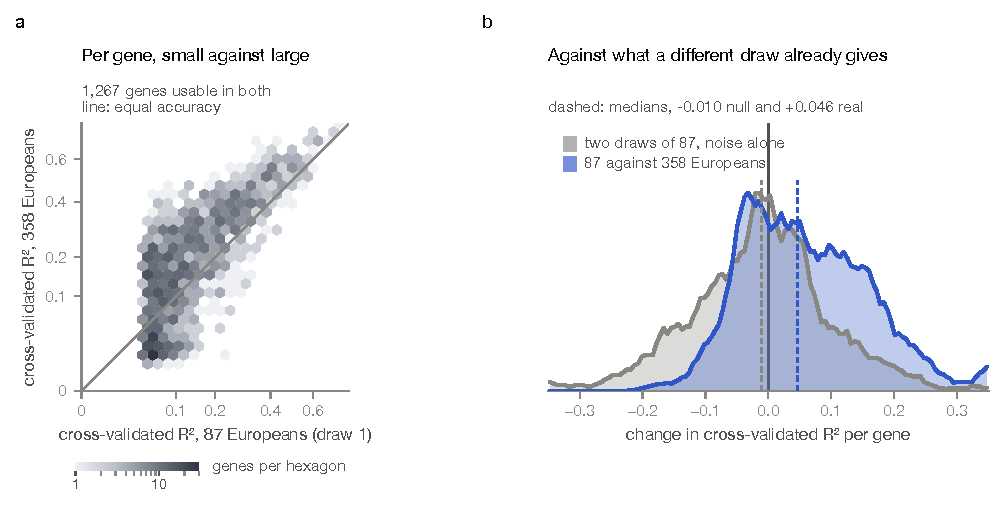
\includegraphics[width=\textwidth]{fig07_sample_size}
\caption{What sample size alone buys. (a) Cross-validated $R^2$ per gene for the 1,267 genes usable both in a draw of 87 Europeans and in all 358, on square-root axes, with the line of equal accuracy. (b) The paired per-gene change from 87 to 358 individuals, drawn against the change between two independent draws of 87, which is what resampling one population at fixed size already gives. Dashed rules mark the two medians.}
\label{fig:samplesize}
\end{figure*}

\subsection{Different Predictors, Similar Weights}
Where the two models selected the same SNP for the same gene, they agreed closely about it (Fig.~\ref{fig:weights}). Across the 2,113 SNP and gene pairs chosen by both, the two weights correlated at $r = 0.589$ and 98.5\% (2,082 of 2,113) carried the same sign. The agreement was not produced by a few large weights: sign agreement stayed above 97\% in every sixth of the weight-size distribution, while the correlation of the weights rose from 0.01 in the smallest sixth to 0.64 in the largest, as expected when small weights are dominated by noise. Neither ancestry systematically received the larger weight, which was European for 40.3\% of shared SNPs. These values are close to those reported for ancestry-specific models trained in brain tissue in a different cohort~\cite{jajoo2025}, which the present result reproduces independently in lymphoblastoid cell lines.

That agreement, however, is conditional on an overlap that is rare (Fig.~\ref{fig:predictors}). Among the same 562 genes, the European models used 21,545 SNPs and the Yoruba models 19,868, yet only 2,113 SNP and gene pairs were common to both, about a tenth of either set. The median model held 31 European SNPs and 27 Yoruba SNPs with a median of one SNP in common, half the genes shared 1.5\% or less of the SNPs used by either model, and 223 of the 562 genes (39.7\%) shared none at all.

The two findings are easy to conflate. A weight correlation near 0.6 describes only the small subset of predictors the two models happen to share, and is compatible with two models that almost never rest on the same variants. Reporting it without the overlap rate beside it overstates how similar the models are.

\begin{figure*}[!t]
\centering
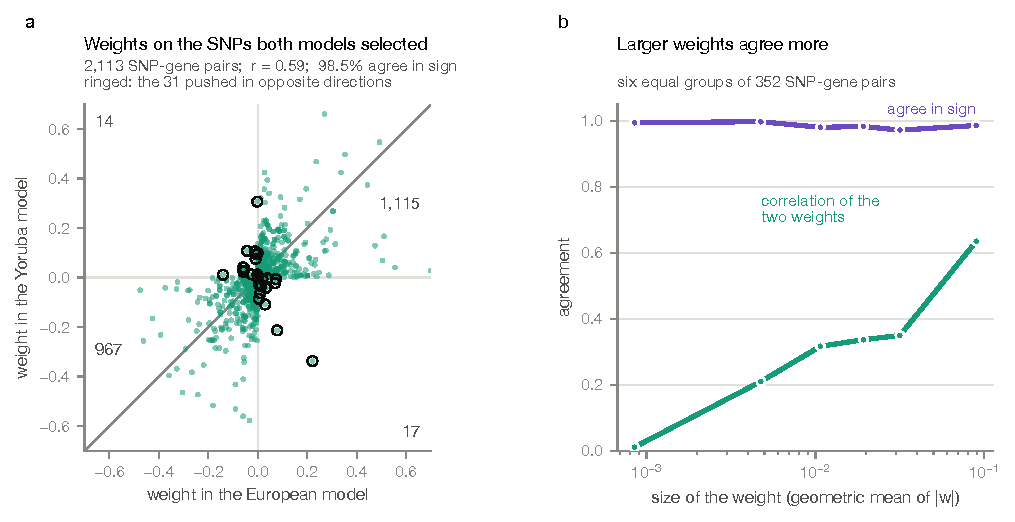
\includegraphics[width=\textwidth]{fig08_weight_agreement}
\caption{Agreement on shared predictors. (a) Every SNP selected by both the European and the Yoruba model for the same gene, placed by the weight each model gave it. The line marks equal weights. Ringed points are the 31 SNPs the two models push in opposite directions, and the corner numbers count the SNPs in each quadrant. (b) Sign agreement and the correlation of the two weights within six equal groups of SNPs, ordered by the size of the weight.}
\label{fig:weights}
\end{figure*}

\begin{figure*}[!t]
\centering
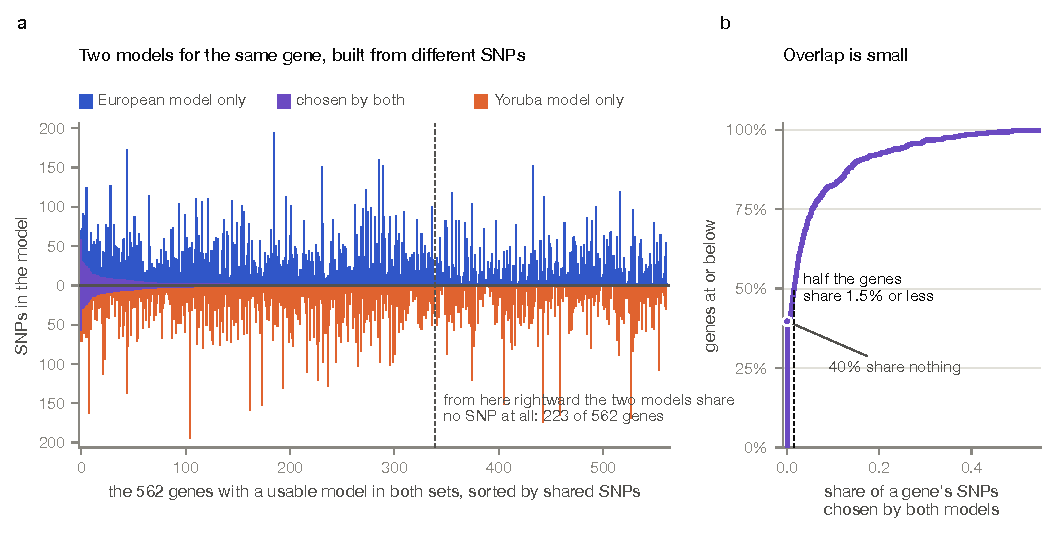
\includegraphics[width=\textwidth]{fig09_shared_predictors}
\caption{The two models are built from different SNPs. (a) One column per gene with a usable model in both sets, sorted by the number of SNPs the two models share. The shared SNPs form the band straddling the axis, the SNPs only the European model chose rise above it, and the SNPs only the Yoruba model chose fall below. To the right of the dashed line the two models share no SNP at all. (b) The share of a gene's SNPs chosen by both models, read cumulatively.}
\label{fig:predictors}
\end{figure*}

\subsection{Where the Disagreement Comes From}
For every gene modelled in both ancestries the gap in genetically regulated variance splits exactly into three parts, and the split summed to the gap to within $10^{-14}$ for all 544 genes where it was defined. The weights term was the largest by a wide margin (Fig.~\ref{fig:triangle}): median absolute components were 0.752 for $\phi_w$, 0.251 for $\phi_D$ and 0.135 for $\phi_R$, and the median gene placed 64\% of its total on the weights, 21\% on allele frequency and 10\% on LD.

Size alone, however, is misleading, and separating the two required a within-ancestry control. Two independent random draws of 87 European individuals differ in nothing but sampling, so by construction their frequency and LD components are exactly zero and their weights component measures training noise alone. Across 699 genes this floor gave a median $|\phi_w|$ of 0.545, against 0.752 between ancestries. Two further pairs of European draws gave 0.556 and 0.606 across 719 and 717 genes, so the floor lies between 0.545 and 0.606, while the cross-ancestry weights term across the three draws lies between 0.731 and 0.773. Restricted to the 356 genes present in both comparisons, counting every gene for which the decomposition was attempted rather than only those with a complete three-way split, the values were 0.446 and 0.633, a ratio of 0.704 (Mann--Whitney $p = 5.8 \times 10^{-6}$). About 70\% of the apparent weights difference between ancestries is therefore reproduced by resampling a single population. The comparison that matters most is blunter still: the noise floor of the weights term, 0.545, exceeds the median frequency and LD components added together, 0.386. This does not depend on which control pair or which European draw is used: the smallest of the three floors, 0.545, is larger than the largest frequency and LD sum across the three draws, 0.395. The largest component of the decomposition is dominated by training noise, while the two smaller ones are not.

Direction separates them further (Fig.~\ref{fig:components}). The weights component was positive for 47.4\% of genes (95\% interval 43.2 to 51.6), indistinguishable from a coin flip, exactly as a noise term should be. The frequency component was positive for 56.6\% (52.5 to 60.8) and the LD component for 44.3\% (40.1 to 48.5), both excluding one half. Allele frequency differences therefore raise the genetically regulated variance in the Yoruba sample more often than not, and LD differences lower it, while the largest component points in no consistent direction at all.

Two further checks support reading the components as what they are named. Each tracks its own genotype quantity: $|\phi_D|$ correlated with weighted allele frequency divergence at Spearman $+0.303$ and $|\phi_R|$ with LD divergence at $+0.298$, while $|\phi_w|$ tracked neither ($-0.031$ and $-0.131$). Across two independent European draws compared against the same Yoruba sample, $\phi_D$ was also the most reproducible component per gene (Spearman $+0.835$), ahead of $\phi_w$ ($+0.676$). The separation is not clean in every draw, however: the cross-term between $|\phi_D|$ and LD divergence was $-0.011$ in the first draw and $+0.157$ in the second, so each component responds mainly, but not exclusively, to its own ingredient.

None of this means ancestry is unimportant. Predictions from two models of the same gene agreed at a median correlation of 0.809 when both came from European draws, but only 0.656 in European individuals and 0.519 in Yoruba individuals when one model came from each ancestry. Two models within one ancestry shared a median of 4 SNPs with 17.5\% sharing none, against a median of 1 and 39.7\% sharing none across ancestries. The ancestry effect is real; it is simply not where the raw size of the weights component suggests.

A single locus shows the anatomy (Fig.~\ref{fig:locus}). At DNAJB7 on chromosome 22, the two models shared 4 of the 76 SNPs either used, the European model predicted Yoruba expression at $r^2 = 0.01$ while the Yoruba model predicted European expression at $r^2 = 0.51$, and the gap decomposed into $\phi_w = +0.08$, $\phi_D = -0.90$ and $\phi_R = -0.35$, summing to $\Delta = -1.17$. Here the frequency term, not the weights, carried the disagreement.

\begin{figure*}[!t]
\centering
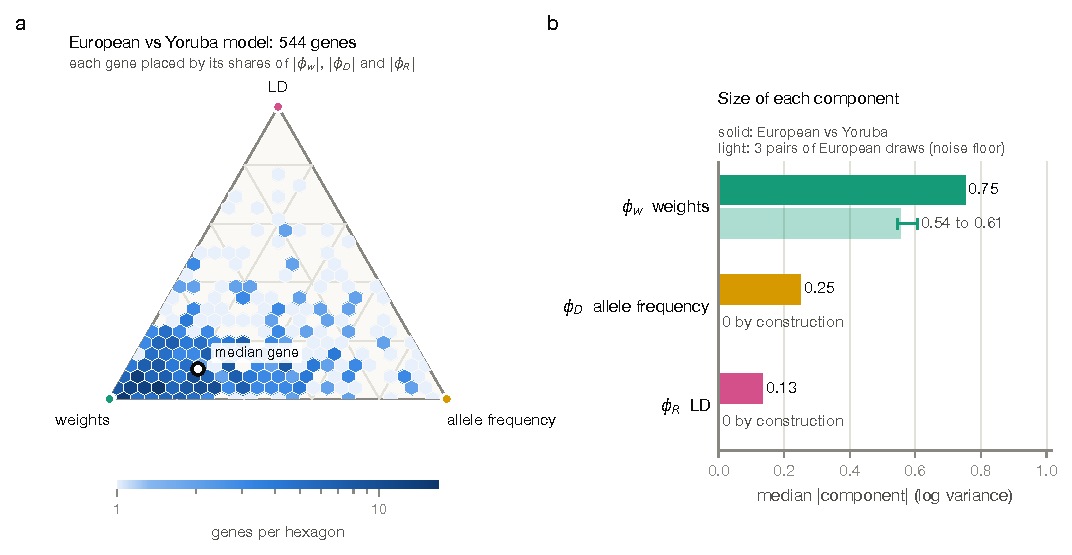
\includegraphics[width=\textwidth]{fig10_decomposition_triangle}
\caption{Where the disagreement between two models comes from. (a) Each gene placed by its shares of $|\phi_w|$, $|\phi_D|$ and $|\phi_R|$, with density on a logarithmic scale and the median gene ringed. (b) Median absolute component between the European and Yoruba models (solid) beside the within-ancestry noise floor (light), where the frequency and LD components are exactly zero by construction. The light weights bar is drawn at the median of the three pairs of independent European draws, and the rule spans them, 0.545 to 0.606.}
\label{fig:triangle}
\end{figure*}

\begin{figure*}[!t]
\centering
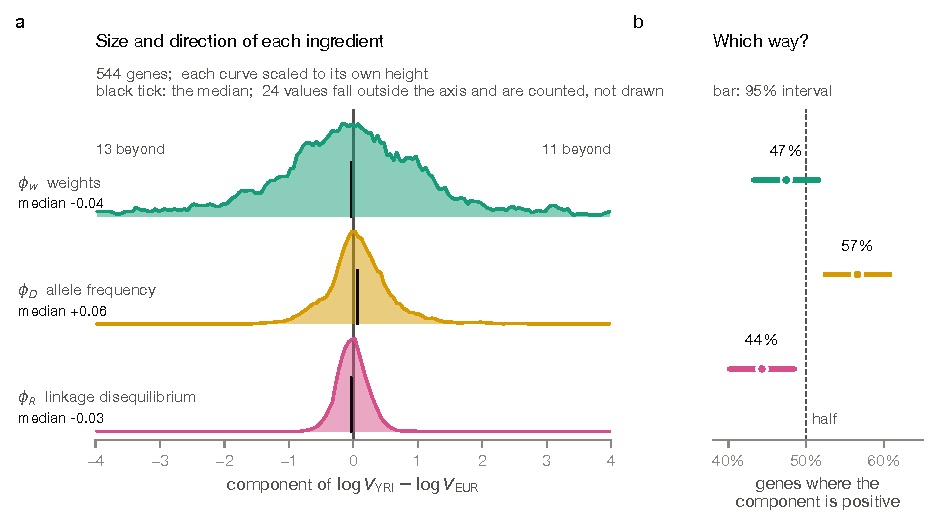
\includegraphics[width=\textwidth]{fig11_component_signs}
\caption{Size and direction of each component. (a) The signed distribution of each component on a common axis, each curve scaled to its own height so the narrow components stay visible, with the median ticked. Values outside the axis are counted at the edge rather than drawn. (b) The share of genes for which each component is positive, with a 95\% interval against a one-half reference. A component reflecting only training noise should sit at one half.}
\label{fig:components}
\end{figure*}

\begin{figure*}[!t]
\centering
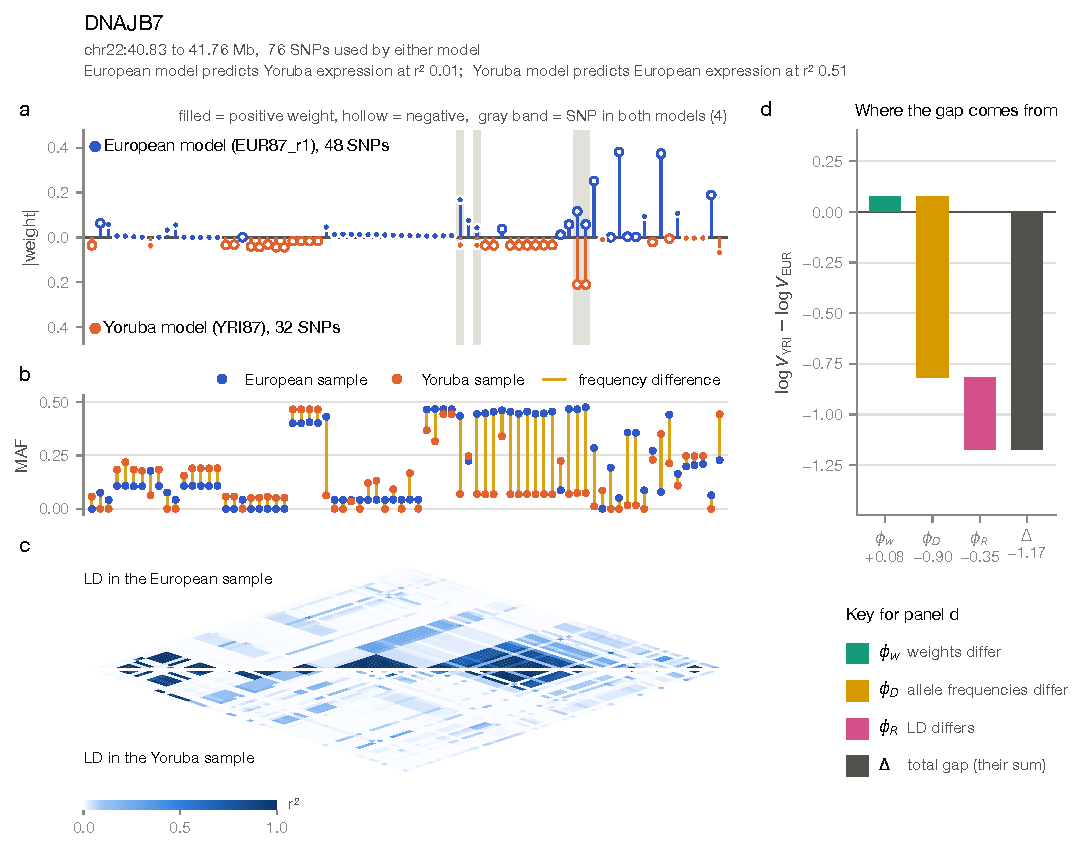
\includegraphics[width=\textwidth]{fig12_locus_DNAJB7}
\caption{Anatomy of one disagreement, at DNAJB7. (a) Model weights, European above and Yoruba below, with grey bands marking the four SNPs both models selected. (b) Minor allele frequency of each model SNP in the two samples, joined by a line whose length is the difference. (c) Pairwise $r^2$ among the same SNPs in each sample. (d) The gap for this gene split into its three components and their sum.}
\label{fig:locus}
\end{figure*}

\subsection{How Much Depends on the Draw}
The decomposition was repeated with three independent draws of 87 European individuals against the same Yoruba sample, so that anything changing between runs is a property of the draw rather than of ancestry (Fig.~\ref{fig:replicates}). At the level of the population the answer is stable: across the three draws the median share of the total ranged from 0.639 to 0.654 for the weights, 0.199 to 0.211 for allele frequency, and 0.101 to 0.103 for LD.

Gene by gene it is not. Pooling all three pairs of draws gives 1,072 comparisons across 458 genes, and the largest of the three components changed for 30.2\% of them (agreement 69.8\%). Of those comparisons, 638 were weights-dominated in both draws, 95 frequency-dominated in both and 15 LD-dominated in both, while 324 switched. The correlation between a gene's weights share in one draw and in another was only Spearman 0.45, with a median absolute change of 0.15. The three pairs agree at 75.4\%, 66.1\% and 68.0\%, so the single pair available earlier understated the instability rather than exaggerating it.

This bounds what the decomposition supports. The population-level statements above are reproducible across draws of the same population. A statement of the form ``for this gene the disagreement is driven by allele frequency'' is not: at this sample size it has roughly a three in ten chance of changing under a different random draw of the same population.

\begin{figure*}[!t]
\centering
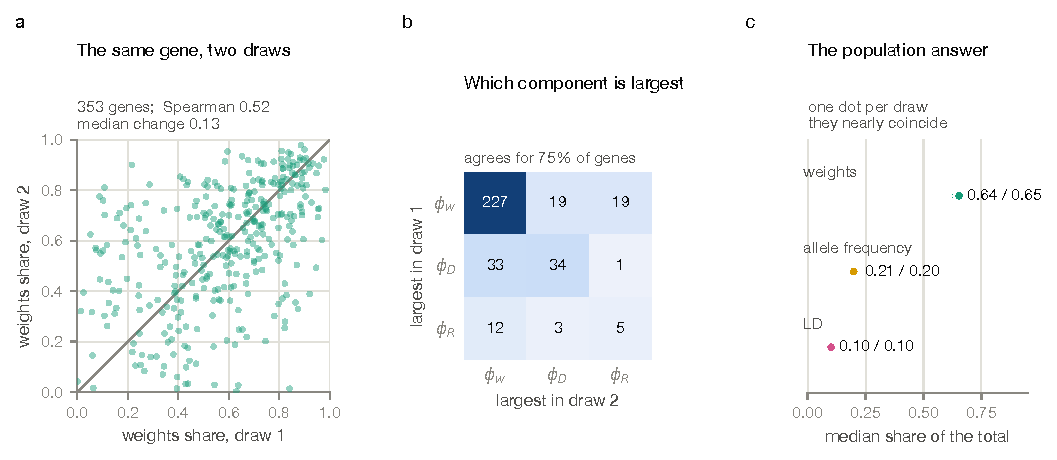
\includegraphics[width=\textwidth]{fig20_replicates}
\caption{How much the answer depends on the draw. The decomposition is run against the same Yoruba sample with three independent random draws of 87 European individuals, and panels (a) and (b) pool all three pairs of draws. (a) Each gene's weights share in one draw against another. (b) Which component is largest for a gene, one draw against another. (c) The median share of each component, one dot per draw.}
\label{fig:replicates}
\end{figure*}

\subsection{What Each Population Can See of the Other's Models}
The SNVs a model relies on are not equally visible in the other population (Fig.~\ref{fig:coverage}). Of 59,376 SNVs in usable Yoruba models, 36.8\% were rare or absent (MAF below 1\%) in the European sample. Of 63,594 SNVs in usable European models, 15.8\% were rare or absent in the Yoruba sample. When a Yoruba-trained model is paired with a European GWAS, the SNVs dropped for missing summary statistics removed a median 22 to 45\% of the model's genetic variance, depending on the trait.
\begin{figure}[!t]
\centering
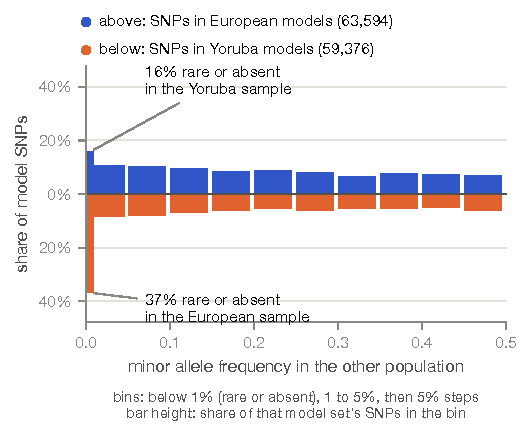
\includegraphics[width=\columnwidth]{fig15_model_snps}
\caption{What each population can see of the other's models. The SNVs selected by usable models, binned by their minor allele frequency in the other population, European models above the axis and Yoruba models below. The leftmost bin holds variants that are rare or absent there.}
\label{fig:coverage}
\end{figure}


\subsection{Crossing Between Populations}
Applying each model set to the other population's individuals gives a direct measure of portability (Fig.~\ref{fig:transfer}). Of the usable European models, 2,272 could be tested in the Yoruba individuals; their median transferred accuracy was a signed $r^2$ of 0.006 and their mean 0.048, with 28.7\% reaching nominal $p < 0.05$. The mean is close to the 0.051 to 0.054 reported for the same populations at comparable sample size~\cite{keys2020}, which supports the pipeline. In the other direction, 2,211 Yoruba models tested in the European individuals gave a median of 0.002 and a mean of 0.063, above the 0.029 to 0.039 reported previously. In both directions the median model transfers almost nothing while the mean is carried by a minority of strongly transferring genes, and roughly 28\% of models predict in the wrong direction in the other population.

Transfer also depends on how well a model works at home, and the dependence is asymmetric. Among models in the top tenth of home accuracy, European models with a median home $R^2$ of 0.371 transferred at a median of 0.151, keeping about 41\%, while Yoruba models with a median home $R^2$ of 0.314 transferred at a median of 0.256, keeping about 82\%. A well-predicted Yoruba model therefore survives the crossing far better than a well-predicted European one, which is consistent with shorter LD in the Yoruba sample forcing the elastic net onto predictors nearer the causal variant, predictors that remain informative in European genomes.

What separates a model that travels from one that does not is mainly whether the two ancestries selected the same variants (Fig.~\ref{fig:portability}). Among the 562 genes modelled in both sets, median cross-population accuracy rose from near zero for genes whose two models share no SNP to about 0.31 for European models and 0.44 for Yoruba models at 17 or more shared SNPs. Holding home accuracy fixed, the partial rank correlation between shared-SNP count and cross-population accuracy was $+0.591$ (95\% bootstrap interval 0.531 to 0.652) for European models and $+0.537$ (0.471 to 0.597) for Yoruba models. Allele frequency divergence had a smaller, direction-specific effect: $-0.155$ ($-0.233$ to $-0.076$) for European models, but $-0.055$ ($-0.139$ to $+0.025$) for Yoruba models, whose interval includes zero. The LD divergence term was positive in both directions, $+0.099$ and $+0.188$, which is the opposite of the naive expectation; because LD divergence is itself correlated with home accuracy and with model size, it is reported here as an association and not interpreted causally.

One quantity was deliberately not used. The apparent drop from home accuracy to cross-population accuracy is negative for 28.5\% of genes in one direction and 47.6\% in the other, because home accuracy is a nested cross-validation estimate while the cross-population figure comes from the final model fitted on all individuals and evaluated in an independent sample. The two are not the same kind of estimate, so their difference is not a clean measure of loss and the analysis uses cross-population accuracy directly instead.

\begin{figure*}[!t]
\centering
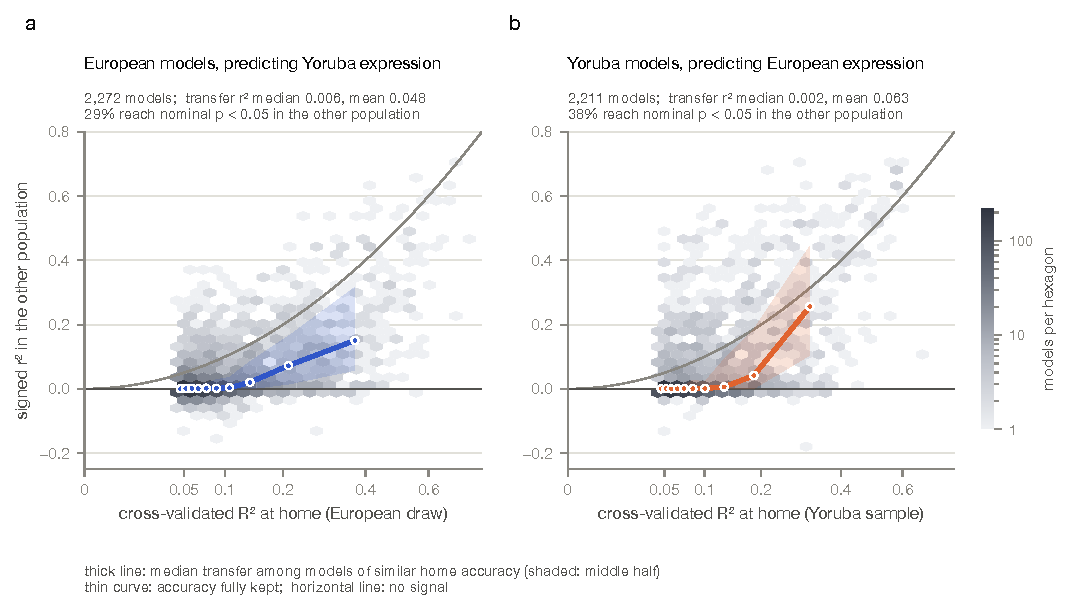
\includegraphics[width=\textwidth]{fig13_transfer}
\caption{How much accuracy survives a crossing. (a) Every usable European model applied to the Yoruba individuals and (b) every usable Yoruba model applied to the European individuals, against the model's cross-validated accuracy at home on a square-root axis. The thick line is the median transferred accuracy among models of similar home accuracy, with the middle half shaded. The thin curve marks accuracy fully kept and the horizontal line marks no signal.}
\label{fig:transfer}
\end{figure*}

\begin{figure*}[!t]
\centering
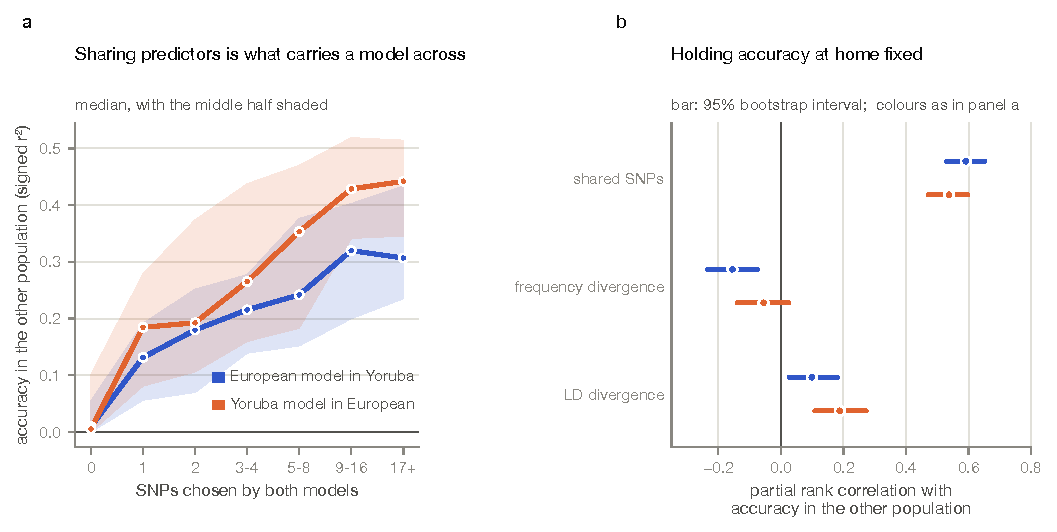
\includegraphics[width=\textwidth]{fig14_portability}
\caption{What carries a model across. (a) Cross-population accuracy against the number of SNPs both models selected for the same gene, in both directions, as a median with the middle half shaded. (b) Partial rank correlation of each predictor with cross-population accuracy, holding the model's accuracy at home fixed, with 95\% bootstrap intervals. Colours are as in panel (a).}
\label{fig:portability}
\end{figure*}

\subsection{Transcriptome-Wide Association by Training Ancestry}
Both model sets were used for summary-statistic TWAS on the same five European GWAS (Figs.~\ref{fig:twas_asd} and \ref{fig:twas_four}). Neither set produced a significant association for autism (2,195 genes tested with European models and 1,986 with Yoruba models), consistent with the smaller size of the autism GWAS relative to the other four. For the remaining disorders, the two model sets returned similar numbers of associations but largely different genes. For schizophrenia, 38 genes were significant with European models and 45 with Yoruba models, of which 8 were significant with both. For bipolar disorder the counts were 17, 14 and 3; for major depression 16, 15 and 3; and for PTSD 8, 9 and none. The strongest associations fell in established loci, including the extended MHC for schizophrenia, NT5DC2 at 3p21.1 for bipolar disorder and major depression, and MAD1L1 and DDX39B for PTSD.
\begin{figure*}[!t]
\centering
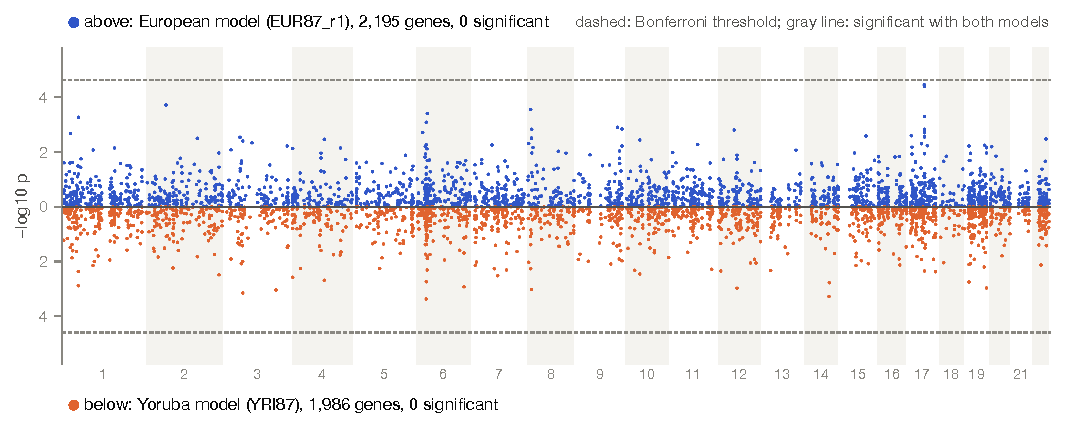
\includegraphics[width=\textwidth]{fig16_mirror_manhattan_ASD}
\caption{Summary-statistic TWAS for autism, with the European model set above each axis and the Yoruba model set below. Dashed lines are the Bonferroni threshold for the genes each set could test.}
\label{fig:twas_asd}
\end{figure*}

\begin{figure*}[!t]
\centering
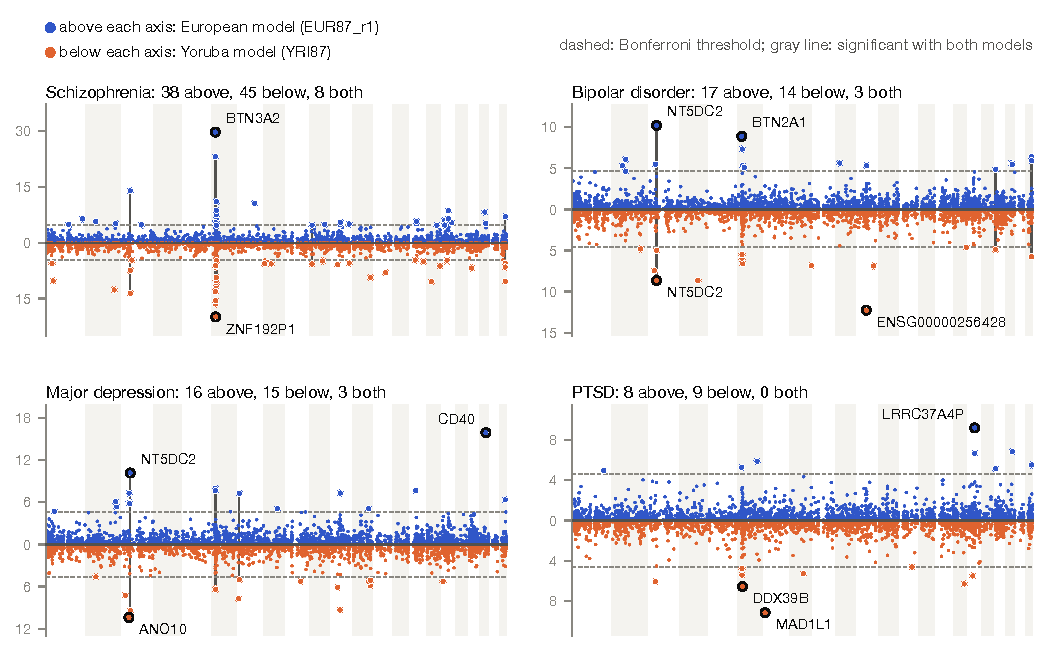
\includegraphics[width=\textwidth]{fig17_mirror_manhattan_four}
\caption{Summary-statistic TWAS for schizophrenia, bipolar disorder, major depression and post-traumatic stress disorder, with the European model set above each axis and the Yoruba model set below. Gray vertical lines connect a gene significant with both model sets.}
\label{fig:twas_four}
\end{figure*}


Part of this limited overlap follows directly from the previous section: a gene can only be significant with both model sets if both produced a usable model for it, and that held for only 562 genes. Separating genes modeled in only one ancestry from genes modeled in both but significant with only one is the purpose of the decomposition that follows.

The equal-size comparison above is the design of this study, but the full European sample shows what the same test does with more usable models. With EUR358, 5,369 genes could be tested for autism, against 2,195 and 1,986 for the two 87-person model sets, and across the four better-powered disorders the number of Bonferroni-significant associations rose from 79 with the European draw of 87 to 183, close to the 2.42-fold increase in usable models. Autism crossed the threshold for the first time, with two associations, but these are not two findings. Both lie on chromosome 17 within 751 kb of each other, the stronger of them is a pseudogene (NSFP1, $p = 1.5 \times 10^{-6}$) and the other is CRHR1 ($p = 6.5 \times 10^{-6}$), and 10 of the 12 most significant autism genes fall between 43.5 and 45.0 Mb on that chromosome. That is a single region of long-range LD read out through many correlated predicted expression traits, not two independent signals, and it is what this kind of test produces when one locus is well tagged.

Calibration was comparable between the two model sets within every trait (Fig.~\ref{fig:qq}). Genomic inflation, European then Yoruba, was 1.25 and 1.08 for autism, 1.86 and 1.89 for schizophrenia, 1.52 and 1.58 for bipolar disorder, 1.78 and 1.82 for major depression, and 1.32 and 1.42 for post-traumatic stress disorder. Values above one are expected for association testing on predicted expression from large polygenic GWAS, because predicted expression is correlated among nearby genes and many genes are genuinely associated. The comparison that matters here is between the two model sets, which are inflated to a similar degree within each trait, and autism, with much the smallest GWAS, is the least inflated.

\begin{figure*}[!t]
\centering
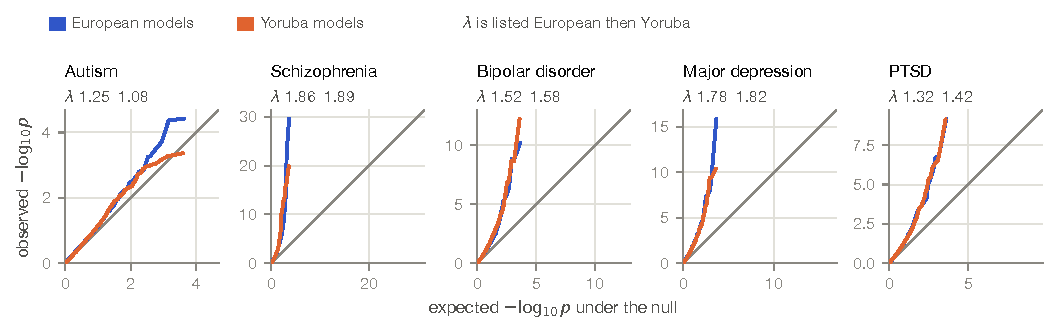
\includegraphics[width=\textwidth]{figS1_qq}
\caption{Calibration of the association tests. Observed against expected $-\log_{10} p$ under the null for each trait, with the European and Yoruba model sets drawn together and the null diagonal marked. Genomic inflation $\lambda$ is printed per panel, European then Yoruba. Each panel carries its own scale because the observed range differs by almost an order of magnitude between traits.}
\label{fig:qq}
\end{figure*}

\subsection{Why an Association Is Ancestry-Specific}
Across the four disorders with any signal, 129 gene and trait associations reached Bonferroni significance with one model set and not the other: 29 European-only and 37 Yoruba-only for schizophrenia, 13 and 10 for bipolar disorder, 13 and 11 for major depression, and 8 and 8 for post-traumatic stress disorder. Autism produced none with either set.

The decomposition can only speak to a minority of these (Fig.~\ref{fig:specific}). An association is ancestry-specific either because the two ancestries built different models of the same gene, in which case the three components are defined, or because the other ancestry never produced a usable model for that gene at all, in which case there is nothing to decompose. The second case accounted for 98 of the 129 associations, 76.0\%. Among the 31 where both models existed, the weights term was the largest component for 27 and allele frequency for 4; LD was largest for none.

Two conclusions follow, and they qualify a common reading of ancestry-specific results. First, at this sample size the dominant reason an association appears with one ancestry's models and not the other is not that the models disagree, but that only one of them exists. Second, among the associations where a comparison is possible, the component that usually dominates is the one the noise floor showed to be largely training noise, and the component most often invoked as the explanation, allele frequency, dominates 4 of 129. A claim that ancestry-specific associations are mostly frequency-driven can only be tested on genes modelled in both ancestries, which is a minority of them here.

\begin{figure*}[!t]
\centering
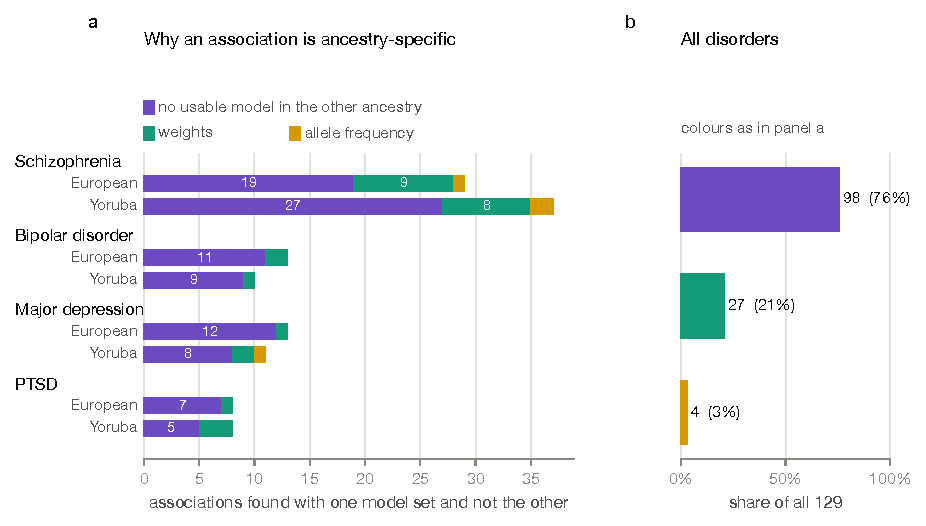
\includegraphics[width=\textwidth]{fig18_specific_hits}
\caption{Why an association is ancestry-specific. (a) For each disorder and each model set, the associations found with that set and not the other, split by whether the other ancestry produced a usable model for the gene at all and, where it did, by the largest component of the decomposition. (b) The same 129 associations pooled across disorders.}
\label{fig:specific}
\end{figure*}

Genes reaching significance for more than one disorder were few, and mostly seen by one ancestry only (Fig.~\ref{fig:crossdis}). Sharing was highest between schizophrenia and bipolar disorder, at 8 genes with European models and 7 with Yoruba models, and fell to 1 or 2 for the pairs involving post-traumatic stress disorder. Five genes reached three or more disorders. NT5DC2 was the only one recovered by both model sets; BTN3A2, CD40 and BTN2A1 reached three or more disorders with European models alone, and ZNF192P1 with Yoruba models alone. The pattern at the level of individual genes matches the pattern across all associations: the two ancestries produce comparable numbers of findings, and largely different ones.

\begin{figure*}[!t]
\centering
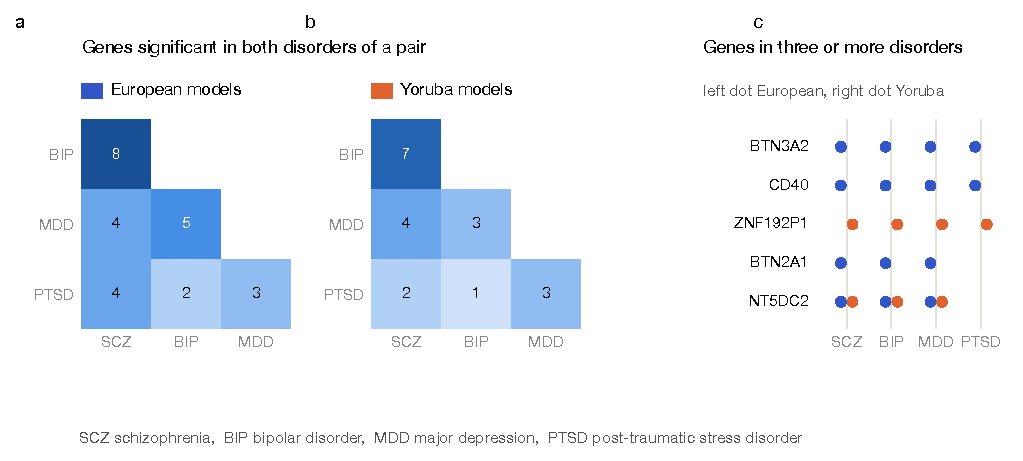
\includegraphics[width=\textwidth]{fig19_cross_disorder}
\caption{Genes shared across disorders. (a, b) The number of genes reaching Bonferroni significance for both disorders of each pair, for the European and the Yoruba model set. (c) Every gene significant in three or more disorders, with a dot per model set that found it.}
\label{fig:crossdis}
\end{figure*}

\section{Discussion}
This study set out to ask not how much accuracy is lost when a gene expression model crosses ancestries, which is established, but which of three ingredients accounts for the disagreement. The decomposition gives an exact answer per gene, and the answer is not the one the raw component sizes suggest.

Taken at face value, the weights term dominates: it is three times the size of the frequency term and six times the LD term, and it holds about 64\% of the median gene's total. Measured against a within-ancestry control, most of that is an artifact of training. Two independent draws of 87 European individuals, which differ by sampling alone, reproduce roughly 70\% of the apparent cross-ancestry weights difference. The noise floor of the weights term exceeds the frequency and LD terms added together. A study reporting only the raw decomposition would conclude that ancestry-specific regulatory effects are the main driver of model disagreement, and that conclusion would be largely an artifact of fitting elastic net to 87 individuals.

The two smaller components behave the opposite way. Neither has any within-ancestry floor, because two draws of one population share a frequency vector and an LD matrix by construction. Both point in consistent directions across genes, each responds mainly to the genotype quantity it is named for, and the frequency component is the most reproducible of the three across independent training draws. Small and systematic is more informative here than large and symmetric.

The practical consequences appear in two places. First, whether a model survives a crossing is decided mostly by whether the two ancestries selected the same variants, far more than by how divergent those variants are in frequency or LD. Second, and more pointedly for association studies, the dominant reason a transcriptome-wide association is found with one ancestry's models and not the other is not that the two models disagree. In 76\% of cases the other ancestry produced no usable model for that gene at all. Among the minority where a comparison is possible, allele frequency is the largest component for 4 of 129 associations. The common summary that ancestry-specific associations are mostly frequency-driven can only be assessed on genes modelled in both ancestries, and at this sample size those are a minority.

The asymmetry between directions deserves note. Well-predicted Yoruba models kept about 82\% of their accuracy in European individuals, while well-predicted European models kept about 41\% in Yoruba individuals. Shorter LD in the Yoruba sample forces the elastic net toward predictors closer to the causal variant, and such predictors remain informative in a population with longer haplotypes, whereas the reverse does not hold. This is a mechanistic hypothesis consistent with the LD measurements here rather than something the data demonstrate directly, and it suggests that training in the population with shorter LD may yield more portable models at equal sample size.

\subsection{Limitations}
The expression data are lymphoblastoid cell lines, not brain, so the transcriptome-wide association results are cell-line based and are labelled that way throughout. The decomposition itself is a property of model weights and population genotypes and does not depend on tissue, but which genes are modelled well certainly does.

Sample size is the binding constraint. At 87 individuals per training set the elastic net reaches a usable model for roughly one gene in nine, and the weights component is dominated by training noise. The within-ancestry floor quantifies that rather than removing it. A larger Yoruba reference panel, not a better estimator, is what would change these numbers.

All five GWAS are European, so the association analysis asks only whether Yoruba-trained models detect signal in European samples. It cannot address whether either model set performs well in African-ancestry disease cohorts, which is the question that matters most for equitable application.

Weighted Fst here is a weighted mean of per-SNP values over the variants a model uses, and those variants passed a minor allele frequency floor of 0.05 in the training sample, which excludes the most strongly differentiated variants by construction. The ratio-of-averages estimator is generally preferred for averaging Fst, so the values reported here should be read as a model-weighted summary rather than a genome-wide figure. The LD divergence term is correlated with both model size and home accuracy, so its positive association with cross-population accuracy is reported as an association only.

Comparing a nested cross-validation estimate at home with a final-model estimate abroad is not a like-for-like comparison, which is why the drop between them is not used as an outcome anywhere in this study.

The decomposition is a reliable population-level summary but not a per-gene one. Repeating it with three independent draws of 87 European individuals changed the largest of the three components for 30.2\% of the 1,072 pooled comparisons, and a gene's weights share moved by a median of 0.15 between draws. Individual genes should therefore not be labelled frequency-driven or weight-driven at this sample size, and none of the conclusions here rest on a single gene.

Finally, the component separation is not perfect. The cross-term between the frequency component and LD divergence was near zero in one European draw and $+0.157$ in a second, so the components should be read as responding mainly, not exclusively, to their own ingredients.

\section{Conclusion}
When two ancestry-specific expression models disagree about a gene, the disagreement can be split exactly into a weights term, an allele frequency term and an LD term. Doing so on GEUVADIS at equal sample size shows that the largest term is the least informative. The weights term is three times the size of the frequency term, but two independent draws of the same European population reproduce about 70\% of it, and its within-ancestry noise floor exceeds the frequency and LD terms combined. The frequency and LD terms are small, have no within-ancestry floor by construction, point in consistent directions, and each responds mainly to the genotype quantity it is named for.

For association studies the practical finding is simpler still. Whether a model survives a change of population is decided mostly by whether the two ancestries selected the same variants, and at 87 training individuals the usual reason a transcriptome-wide association appears with one ancestry's models and not the other is that the other ancestry produced no usable model for that gene at all. Reporting a decomposition of cross-ancestry disagreement without a within-ancestry control will overstate the role of ancestry-specific regulatory effects, and the control costs nothing beyond a second random draw of the population already in hand.

\section*{Data and Code Availability}
All data used in this study are public. Gene expression came from the GEUVADIS project, ArrayExpress accession E-GEUV-1, using the released gene-level RPKM matrix for 462 lymphoblastoid cell lines. Genotypes came from the 1000 Genomes Project phase 3 release distributed as a PLINK 2 resource on GRCh37; 445 of the 462 individuals with expression data are present in that release and form the analytic sample. Summary statistics came from the Psychiatric Genomics Consortium: the iPSYCH-PGC autism meta-analysis, the PGC3 schizophrenia European meta-analysis, the PGC bipolar disorder meta-analysis, the PGC major depression meta-analysis excluding 23andMe, and the PGC post-traumatic stress disorder European meta-analysis. File names, download dates, sizes and MD5 checksums for every input are recorded in the repository.

Analysis code, including the training pipeline, the decomposition, the summary-statistic association implementation and every figure script, is available in the project repository. Each figure in this paper is produced by a named script from recorded intermediate files, and the reference list is checked against Crossref by a script that verifies the title, first author, year and journal of every entry before the manuscript is compiled.

\bibliographystyle{IEEEtran}
\bibliography{references}

\end{document}
